
\chapter{Trabajos Relacionados\label{chap:Trabajos-Relacionados}}

El enfoque propuesto básicamente es un proceso de aprendizaje de máquina
que incluye una herramienta para recolectar mediciones de performance
en Android (y Java), y otra herramienta para entrenar y evaluar modelos
de predicción con diferentes técnicas de aprendizaje automático. Por
lo tanto, este capítulo se dividirá en dos secciones para describir
en la sección \ref{sec:Herramientas-de-benchmarks-para-Android} un
conjunto de herramientas sobre benchmarks en Android y en la sección
\ref{sec:Predicci=0000F3n-de-propiedades-no-funcionales-con-aprendizaje-de-m=0000E1quina}se
presentarán algunos trabajos ya realizados que llevan a cabo la predicción
de atributos a través de modelos.


\section{Herramientas de benchmarks para Android\label{sec:Herramientas-de-benchmarks-para-Android}}

Las herramientas de benchmarking han ido incrementando su popularidad
ya que ofrecen a los usuarios la posibilidad de analizar a fondo todos
los aspectos de un dispositivo android arrojando datos numéricos acerca
de la potencia, eficiencia y capacidad de los mismos. La recolección
y conocimiento de estas propiedades no funcionales son relevantes
y necesarios al momento de determinar cuál dispositivo será el más
adecuado para satisfacer la carga de trabajo esperada. A continuación
se describen algunas herramientas de benchmarking. 


\subsection{Performance Monitors de Android \label{sub:Performance-Monitors-de-Android }}

Es una herramienta integrada en el ambiente de desarrollo \emph{Android
Studio} y cuenta con varias sub herramientas que proveen información
en tiempo real sobre la aplicación, estos datos capturados se almacenan
en archivos para luego analizarlos en diferentes vistas. Pueden realizarse
pruebas de rendimiento sobre dispositivos Android conectados directamente
a la aplicación o simulados a través de un emulador, en ambos casos
se debe tener en cuenta que \emph{Android Device Monitor }no puede
ser utilizada. \emph{Android Monitor} utiliza la \ac{VM} del dispositivo
o emulador dependiendo de la versión del sistema Android. 

A través de cinco vistas diferentes se accede a la información sobre
la aplicación evaluada. \emph{LogCat} muestra en detalle las excepciones
emitidas por la aplicación, útil para detectar y eliminar errores
que mejoren el funcionamiento de la aplicación. 

Durante la ejecución de la aplicación también hay seguimiento gráfico
del consumo de memoria junto con los eventos de garbage collection
(\emph{GC}) para detectar relaciones entre éstos y los puntos de latencia,
el porcentaje total de uso de \ac{CPU} (incluyendo todos los núcleos)
que se utiliza en modo de usuario y modo kernel, una visión general
de la performance de la interfaz incluyendo la cantidad de tiempo
que le lleva al thread preparar, procesar y ejecutar los comandos
gráficos, y finalmente, el seguimiento de cada solicitud de red que
es realizada, al mismo tiempo que permite controlar la manera y el
momento en que se llevan a cabo las transferencias de datos en la
aplicación para optimizar el código subyacente de manera apropiada. 

Adicionalmente, la herramienta \emph{Android Monitor} provee funciones
para examinar información relevante sobre el estado de los servicios
del sistema, y permite realizar capturas y videos de la pantalla. 


\subsection{Benchit\label{sub:Benchit}}

\emph{Benchit} es una librería Open Source implementada en lenguaje
Java de Benchmarking para Android. El uso de esta herramienta se hace
mediante un repositorio maven llamado \emph{JitPack} (accedido a través
de la URL \emph{https://jitpack.io}) el cual contiene el proyecto
\emph{T-Spoon/Benchit}. JitPack puede utilizarse tanto en proyectos
Android como en la \ac{VM} de Java y provee artefactos listos para
su uso como archivos jar y aar. El proyecto ha sido configurado para
ejecutarse a partir de la versión 8 de Android. 

Benchit es un framework rápido y sencillo ya que permite añadir benchmarks
en áreas de código deseadas para determinar el tiempo o latencia de
la operación. Una forma sencilla de utilizar esta librería es a través
de iteraciones sobre una misma sección de código. De esta forma, con
cada iteración, la herramienta va almacenando el tiempo de ejecución
del código (diferencia entre el tiempo de comienzo y tiempo de fin).
Al término de las iteraciones, se podrá observar el resultado en la
herramienta LogCat mostrando tres propiedades: promedio, rango y desviación
estándar. La herramienta, también provee la posibilidad de realizar
comparaciones entre todos o algunos benchmarks del código mostrando
los resultados de manera ordenada. Esta opción es útil, por ejemplo,
al momento de comparar el desempeño de varios algoritmos o sentencias
que realicen la misma acción de forma diferente. 


\subsection{Google Caliper \label{sub:Google-caliper}}

\emph{Google Caliper} es un framework open source para implementar,
ejecutar y visualizar resultados de microbenchmarks en aplicaciones
Java, aunque brinda soporte para proyectos android accediendo a través
de la rama de la versión 0.5 ya que la rama 1.0 no funciona correctamente
en Android. Existen dos alternativas de acceso al proyecto a través
del repositorio maven o el repositorio git. Caliper permite obtener
diferentes medidas del código Java, principalmente microbenchmarks,
pero también tiene soporte para otros tipos de medidas incluyendo
memoria disponible, ocupada, u otras medidas arbitrarias de dominio
específico como por ejemplo el radio de compresión. 


\subsection{Java Microbenchmark Harness\label{sub:Java-Microbenchmark-Harness}}

Java Microbenchmark Harness (\emph{JMH}), es una herramienta que facilita
la implementación de benchmarks en forma correcta. El término correcto
hace alusión a las optimizaciones que tanto la máquina virtual como
el hardware subyacente aplican sobre el código durante la ejecución
de los benchmarks y que no se aplican en sistemas de producción real,
infiriendo en conclusiones erróneas sobre el rendimiento. \emph{JMH}
fue diseñada por los mismos desarrolladores de la máquina virtual
de Java posibilitando la construcción, ejecución y análisis de benchmarks
no sólo escritos en lenguaje Java sino en otros lenguajes soportados
por la máquina virtual. 

La librería \emph{JMH} ofrece cinco tipos de medidas sobre el código
(modos) especificados por medio de anotaciones Java. 
\begin{description}
\item [{Throughput}] mide el número de operaciones por segundo, un estimativo
sobre la cantidad de veces por segundo que el componente podría ser
ejecutado. 
\item [{Average~time}] mide el tiempo promedio que el componente requiere
para ejecutarse.
\item [{Sample~time}] mide el tiempo efectivo que el componente requirió
en ejecutarse, incluyendo tiempo máximo y mínimo. 
\item [{Single~Shot}] mide el tiempo de ejecución de un simple método
benchmark. 
\item [{All}] computa y retorna todas las mediciones anteriores. 
\end{description}

\subsection{JMeter\label{sub:JMeter}}

\emph{JMeter} es una herramienta Open Source diseñada por Apache e
implementada completamente en lenguaje Java para realizar pruebas
de carga y medidas de rendimiento. Apache JMeter puede utilizar para
simular un gran volumen de carga en un servidor o grupo de servidores
y en la red y probar su resistencia o analizar el rendimiento general
bajo diferentes tipos de carga. En un principio, fue diseñada para
realizar pruebas de rendimiento sobre aplicaciones Web pero luego
ha sido extendida a otras funciones para cubrir diferentes categorías
de testing, tal es el caso de los análisis de carga, de funcionalidad,
desempeño, regresión, entre otros. JMeter es una aplicación de escritorio
con una interfaz gráfica amigable para el usuario. Puede ser ejecutada
bajo cualquier entorno o estación que acepte la máquina virtual de
Java como es el caso de los sistemas operativos Windows, Linux y Mac.

A grandes rasgos, la herramienta simula un grupo de usuarios que envían
peticiones a un servidor y retorna un conjunto de estadísticas sobre
el desempeño y funcionalidad por medio de gráficos, tablas, etc, tanto
sobre recursos estáticos y dinámicos. Al tratarse de un framework
basado en java, el único requerimiento es la instalación de la herramienta
\ac{JDK} a partir de la versión 6. 

El cuadro comparativo \ref{tab:benchmarks-tools} resalta las propiedades
o medidas que pueden realizar las herramientas antes mencionadas y
los componentes sobre los cuales realizan las mediciones.

\begin{table}
\begin{centering}
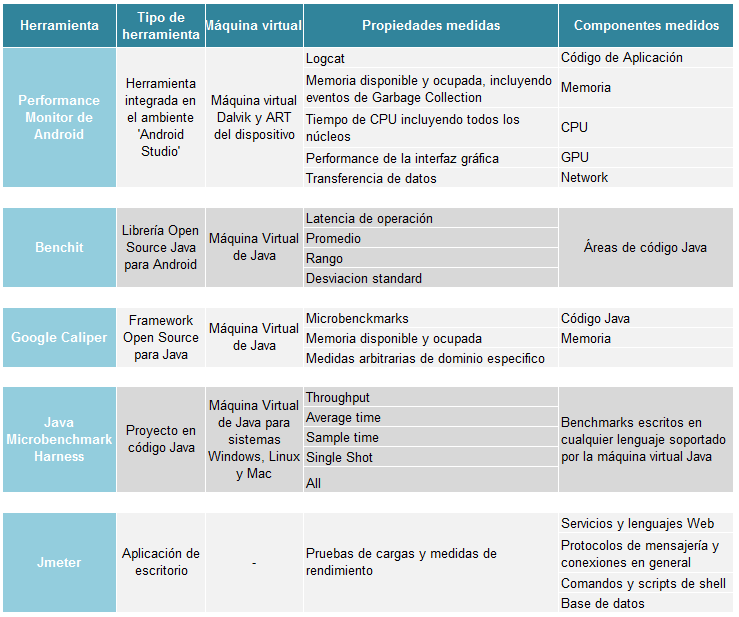
\includegraphics[scale=0.55]{C:/Users/usuario/Tesisworkspace/Tesis_Standalone/tesis/images/benchmarks_tools}
\par\end{centering}

\caption{Información resumida de herramientas de pruebas de performance para
aplicaciones Android y servicios Web.}
\label{tab:benchmarks-tools}
\end{table}



\section{Predicción de propiedades no funcionales con aprendizaje de máquina
\label{sec:Predicci=0000F3n-de-propiedades-no-funcionales-con-aprendizaje-de-m=0000E1quina}}

La predicción de propiedades no funcionales ha contribuido a los arquitectos
de software en la evaluación de sus sistemas durante la etapa de diseño,
y guiar las decisiones respecto a los componentes que deben integrarse
a la arquitectura del sistema de acuerdo a los requerimientos de calidad
esperados. Diferentes trabajos han recurrido al uso de técnicas de
aprendizaje de máquina para construir modelos de predicción de performance
y otros atributos de calidad dinámicos. Hutter, Xu y Hoos \citep{Hutter2014}se
han referido a estos modelos como modelos empíricos de performance
(\emph{EPM} por sus siglas en inglés) ya que requieren la recolección
de mediciones empíricas sobre los componentes. La principal aplicación
de estos modelos probablemente es el problema de selección de algoritmos,
introducido en 1976 por John R. Rice \citep{Rice1976}. Este problema
consiste en seleccionar el algoritmo, o configuración de algoritmo,
de un portafolio de alternativas que minimice el tiempo de respuesta,
según la instancia de datos de entrada. La predicción del tiempo de
respuesta ha sido abordada con éxito usando técnicas de aprendizaje
supervisado, principalmente de regresión \citep{Hutter2014}. En estos
trabajos, los datos empíricos de entrenamiento son obtenidos en contextos
de ejecución controlados, para enfocarse en la correlación entre la
propiedad a predecir y las propiedades de los parámetros de entrada
del componente o algoritmo. Una limitación de estos modelos es que
no generalizan la predicción de las propiedades de performance al
contexto de ejecución, es decir, no consideran características del
dispositivo y el ambiente de ejecución que influyen sobre el desempeño
del componente, como su capacidad de cómputo y la disponibilidad de
recursos. 

Este capítulo describe trabajos que inducen al desarrollo de una herramienta
capaz de generalizar cualquier característica propia del componente
de ejecución como así también del entorno donde se ejecuta para la
aplicación de la técnica de aprendizaje de máquina que resulte la
más adecuada para la predicción. Está organizado de la siguiente manera:
la sección \ref{sub:Predicci=0000F3n-de-precisi=0000F3n} presenta
tres estudios sobre algoritmos de optimización que abarcan la predicción
de otro de los indicadores más importantes, como lo es la precisión
y en la sección \ref{sub:Predicci=0000F3n-sobre-Servicios} presenta
dos estudios de propiedades dinámicas sobre Servicios Web. 


\subsection{Predicción de precisión sobre algoritmos de optimización. \label{sub:Predicci=0000F3n-de-precisi=0000F3n}}

Los modelos de predicción no sólo se utilizan para estimar el tiempo
de respuesta del desempeño de los componentes, sino también para estimar
otras propiedades. Mark Roberts, Adele Howe y Landon Flom \citep{Roberts07learnedmodels}
han construido dos modelos para la predicción del tiempo de respuesta
y para la probabilidad de éxito de diferentes algoritmos de planeamiento
utilizando técnicas de aprendizaje de máquina incluidas en la librería
Weka. Para el aprendizaje fueron utilizados 4726 benchmarks, problemas
o instancias para ejecutarse sobre 28 algoritmos de planeamiento conocidos.
Por cada algoritmo y cada problema se registra si un plan fue encontrado
(éxito) a través de los valores verdadero o falso y se registra el
tiempo (en segundos) requerido en completar la ejecución. Ya que cada
algoritmo define su propia forma en que un resultado es exitoso o
no, de forma automática obtienen las métricas de precisión porcentuales
sobre la salida. 

Otros autores (Mersmann; Bischl; Trautmann; Wagner; Bossek y Neumann
\citep{Mersmann_anovel}) predicen la optimalidad o razón de aproximación
de algoritmos para el problema del viajante utilizando una técnica
de regresión no lineal llamada \emph{MARS}, por sus siglas en inglés.
El modelo \emph{MARS} se aplicó con éxito para predecir la calidad
de aproximación del algoritmo de búsqueda local llamado 2-opt independiente
del tamaño de la instancia sobre la base de las características de
los casos generados con una precisión muy alta. Se cree firmemente
que debiera ser sencillo aplicar la misma metodología a otros algoritmos
y utilizar estos modelos para derivar una estrategia para el problema
de selección de algoritmos en el contexto de los problemas \ac{TSP}.

Finalmente, el trabajo desarrollado por los autores Beveridge, Givens,
Phillips y Draper \citep{Beveridge2009} se analiza la precisión de
tres componentes diferentes para el reconocimiento de rostros en imágenes,
utilizando una técnica de regresión lineal denominada GLMM, por Generalized
Linear Mixed Models. 


\subsection{Predicción sobre Servicios Web \label{sub:Predicci=0000F3n-sobre-Servicios}}

La predicción de propiedades dinámicas de servicios Web, como su tiempo
de respuesta, throughput y probabilidad de fallos, es más compleja
de abordar con respecto a componentes locales ya que depende del estado
de la infraestructura de red y el proveedor del servicio, que no se
puede monitorear desde el dispositivo cliente. Un enfoque ingenioso
para abordar este problema fue propuesto en el articulo de Zheng\citep{Zheng2013}.
En este trabajo, los autores se basan en la premisa de que las propiedades
de performance de los servicios Web varían respecto a características
del contexto como la ubicación geográfica y el momento del día y la
semana en el que se realiza una solicitud al servicio. De esta forma,
recolectan la información del consumo de servicios de múltiples clientes
alrededor del mundo para generalizar modelos de predicción. Este enfoque
es conocido como predicción colaborativa ya que los datos empíricos
de entrenamiento son brindados por múltiples nodos de manera distribuida.
Los autores llevaron a cabo un experimento a gran escala que involucró
más de 30 millones de invocaciones a servicios Web en más de 80 países,
por usuarios distribuidos en más de 30 países. La observación experimental
indica que diferentes usuarios pueden tener diferentes experiencias
de uso sobre el mismo servicio, influenciados por la conexión de red
y los ambientes heterogéneos entre usuarios y proveedores. Los datos
se encuentran disponibles públicamente y han sido utilizados en varios
trabajos para la construcción y comparación de modelos de performance
con diferentes técnicas de aprendizaje de máquina \citep{Albu2013}\citep{Kumar2015}. 
